\chapter{Практическая часть}
\label{cha:ch_2}

\section{Проектирование архитектуры}
% Какая задача поставлена
На основе данной задачи выделяются следующие подзадачи, которые необходимо
выполнить, для успешной реализации инфраструктуры:
\begin{enumerate}[label=\arabic*.]
    \item Описать возможные процессы взаимодействия между компонентами системы.
        Удобно произвести описание с помощью UML диаграммы;
    \item Смоделировать архитектуру приложения: какие компоненты будут
        взаимодействовать друг с другом;
    \item Далее равнозначные задачи, которые не обязательно выполнять
        последовательно: написать файлы запуска и написать кодовую базу для
        запуска каждой из компоненты системы.
\end{enumerate}

Далее рассмотрим каждый из пунктов подробнее, опишем способ реализации,
возникшие проблемы и пути решения.

\section{UML диаграмма}
Для наглядной демонстрации ожидаемого поведения удобно использовать подвид UML диаграмм -- диаграмму активностей.
\begin{figure}[H]
    \centering
    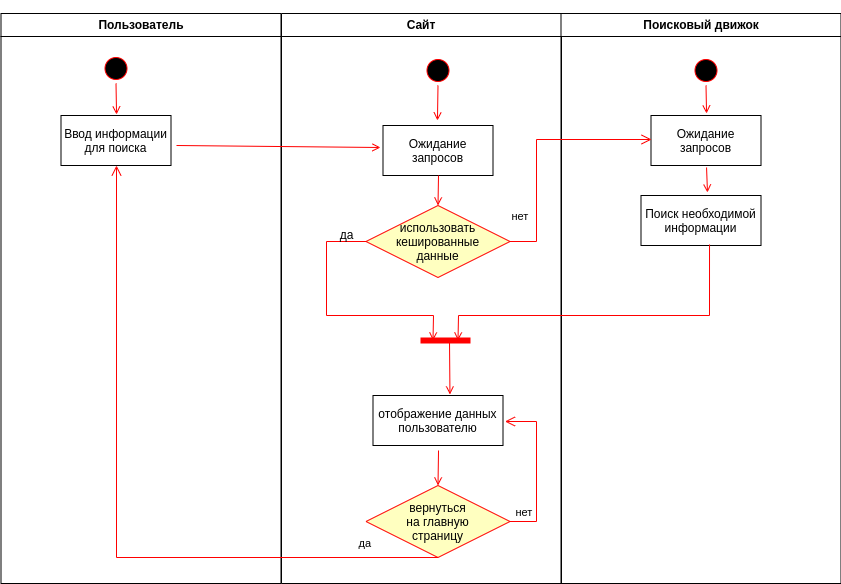
\includegraphics[scale=0.55]{inc/img/activity_diagram.png}
    \caption{Диаграмма активностей для проекта}
\end{figure}

С помощью данной диаграммы можно донести общую концепцию инфраструктуры. Также
на ее основании можно выбрать необходимые для реализации компоненты. Диаграмма
не является точным техническим заданием, а лишь выполняет демонстративную роль.

\section{Архитектура приложения}
После составления UML диаграммы можно определить свойства компонентов и
произвести их выбор.

Для наглядности составим архитектуру всего приложения.
\begin{figure}[H]
    \centering
    
\includegraphics[scale=0.70]{inc/img/structure.png}
    \caption{Архитектура приложения}
\end{figure}

В качестве web-сервера выбран Nginx с его "event based" моделью обработки
входящих соединений, которая обеспечивает быстродействие.

Web-фреймворком выступает Flask, который достаточно легковесный и позволяет
разработчику иметь больше контроля над проектом. Для того, чтобы использовать
Flask вместе с Nginx используется uwsgi.

% TODO: можно еще много чего написать про scrapy и scrapyd: что конкретно
% делают, что конкретно упрощают
Scrapy помогает разработчику извлечь необходимые данные с web-сайтов. Данный
фреймворк написан на Python и имеет открытый исходный код. Содержит в себе
большое количество настроек и достаточно масштабируем "из коробки". В
совокупности со scrapyd позволяет распологать инфраструктуру по поиску на
вычислительных серверах, а также использовать API для просмотра данных.

Для обеспечения доставки сообщений используется kafka (и его модель
Publish-Subscribe). Данный брокер сообщений снимает с приложений нагрузку
связанную с маршрутизацией и отправкой сообщений. Для оркестрации кластеров
kafka используется zookeeper.

В качестве СУБД выбран elasticsearch, т.к. им удобно пользоваться через API
запросы передавая json структуры. Можно создать несколько реплик обеспечив
отказоустойчивость системы. Где каждый узел кластера действует как координатор
для делегирования операций правильному сегменту с автоматической
перебалансировкой и маршрутизацией. Сама СУБД является документоориентированной
что избавляет разработчика от составления схем хранения, хотя для
оптимизированной работы нужно индексировать документы (без схем происходит
автоматически). При продвинутом использовании можно подключить остальные
компоненты системы, например Logstash для работы с логами.

\section{Разработка практических решений}
Спроектировав основную архитектуру и используемые модули можно приступать к
реализации конкретных компонентов.

\subsection{Docker}
\subsection{Docker Compose}
\subsection{Scrapy}
Используя фреймворк Scrapy мы пишем абстрактные классы, называемые web-пауками,
каждый из которых можно настроить. В нем мы пишем логику перехода по ссылкам,
как с ними работать, и какие данные нужно достать со страницы.

Для начала объявляем класс "паука" в папке \verb|spiders| и задаем ему
настройки, относящиеся ко всем паукам как к единому целому:
\begin{itemize}
    \item \verb|name| -- по какому имени можно обращаться к web-паукам как к группе;
    \item \verb|custom_settings| -- общие настройки для web-пауков
\end{itemize}

\begin{verbatim}
class GithubSpider(scrapy.Spider):
    name = "github"
    custom_settings = {
        "lang_mapping": {
            "python": "Python",
        },
    }
\end{verbatim}

Настройки также можно расположить в файле \verb|settings.py|, но было решено
объявить их поближе к самому коду для легкости поиска.

Далее объявляем каким образом будут инициализироваться объекты класса. От имени
и количества входных параметров будет зависить то, какие аргументы будет
принимать консольный интерфейс Scrapy. При инициализации необходимо чтобы каждый
конкретный объект класса имел переменную \verb|start_urls| с которой он начинает
свой путь. Составляем эту переменную, используя функцию \verb|urlencode| вместе
со словарем. Крайне рекомендуется использовать специальные функции для работы с
URL, особенно если составляешь его из входных данных, т.к. должна присутствовать
функциональность экранирования специальных символов. Также проверяем
инициализированны ли входные параметры, и, если нет, то возвращаем текстовое
описание ошибки.
\begin{verbatim}
def __init__(self, topic=None, language=None, *args, **kwargs):
    super(GithubSpider, self).__init__(*args, **kwargs)

    assert topic is not None, "you should provide topic variable via cmd"
    self.topic = topic

    params = { "q": topic, }
    if language is not None:
        params.update({"l": self.custom_settings["lang_mapping"][language]})
    self.start_urls = [f"https://github.com/search?"+urlencode(params)]
\end{verbatim}

% TODO: сделать сноску с примером разбора xpath селектора
% TODO: написать про функции response.follow и response.follow_all
Пишем функцию, которая будет отвечать за переход по страницам поиска (по
страницам пагинации). В ее обязанности входит по каждому найденному репозиторию
вызвать соответствующий обработчик конкретной страницы и перейти на следующие
страницы. Для поиска ссылок для перехода (в более общей задаче -- для поиска
конкретного html элемента) применяется селекторы xpath, которые помогают
разработчику указать по каким правилам должен искаться конкретный элемент. В
данном блоке кода (и во всех функциях парсера) используется ключевое слово
\verb|yield|, которое позволяет вернуть результат вызывающей функции и
продолжить выполнение. В самом конце вызываем для всех найденных ссылок на
репозитории вызываем соответствующий обработчик.
\begin{verbatim}
def parse(self, response):
    # если есть следующая страница, запускаемся на следующей
    next_page = response.xpath('//a[@class="next_page"]/@href').get()
    if next_page is not None:
        # response.follow нативно поддерживает переход по относительным url
        yield response.follow(next_page, callback=self.parse)

    # находим репозитории на текущей странице
    repos_selector = response.xpath('//li[contains(@class, "repo-list-item")]'
                                    '//div[contains(@class, "text-normal")]'
                                    '/a')
    yield from response.follow_all(repos_selector, self.parse_repo)
\end{verbatim}

Далее нужно запарсить каждый отдельный репозиторий. Для этого реализиуем
функцию, которая будет по селекторам xpath находить нужные элементы, например,
язык программирования, популярность. Также в этом блоке кода используется
объявленные раньше общие настройки -- какой язык программирования встречается на
гитхаб, и к какому виду его нужно нормализовать (например c++ может писаться как
c++ или как cpp). В конце возвращаем словарь из данных, которые получили с
обработанной страницы.
\begin{verbatim}
def parse_repo(self, response):
    ### язык кода
    ### берем первый из списка, на проценты не смотрим
    language = response.xpath(
        '//h2[text() = "Languages"]/parent::div/ul/li/a/span/text()').get()
    # если существует конверсия в мой внутренний тип языка, то используем
    # его
    for key, val in self.custom_settings["lang_mapping"].items():
        if language == val:
            language = key
            break

    ### about
    ### у каждого репо есть короткое описание о чем он
    about = response.xpath(
        '//h2[text() = "About"]/parent::div/p/text()').get()

    ### популярность (валидна для гитхаба)
    ### (при выводе для каждого сайта надо нормализовать)
    popularity = response.xpath(
        '//span[contains(@class, "social-count")]/text()').get()

    # change how yield works
    yield {'repo_url': response.url,
            'language': language,
            'about': about,
            'popularity': popularity}
\end{verbatim}

% TODO: подробнее описать что это
Для того чтобы с возвращаемым словарем можно было работать, нужно объявить Data
Class в файле items.py.
\begin{verbatim}
import scrapy

class AlgoSearchItem(scrapy.Item):
    repo_url = scrapy.Field()
    language = scrapy.Field()
    about = scrapy.Field()
    popularity = scrapy.Field()
\end{verbatim}

Чтобы web-пауки могли пересылать свои куда либо еще (кроме базово настроенного
json файла) для начала надо модифицировать файл \verb|pipelines.py|. Пишем
инициализацию начальных переменных из файла настроек. Из него должны читаться
местоположение сервера, на котором находится брокер kafka и сам топик, куда мы
должны писать сообщения
\begin{verbatim}
class AlgoSearchPipeline:
    def __init__(self, kafka_bootstrap_server, kafka_topic):
        self.kafka_bootstrap_server = kafka_bootstrap_server
        self.kafka_topic = kafka_topic

    @classmethod
    def from_crawler(cls, crawler):
        return cls(
            kafka_bootstrap_server=crawler.settings.get('KAFKA_BOOTSTRAP_SERVER'),
            kafka_topic=crawler.settings.get('KAFKA_TOPIC')
        )
\end{verbatim}

Пишем функцию, которая запускается вместе с web-пауками. В ней создаем объект
класса KafkaProducer, который позволяет инкапсулировать в себя всю логику
сериализации сообщений.
\begin{verbatim}
def open_spider(self, spider):
    self.producer = KafkaProducer(
        bootstrap_servers=[self.kafka_bootstrap_server],
        value_serializer=lambda val: json.dumps(val,ensure_ascii=False).encode('utf-8'))
\end{verbatim}

Добавляем логику собственно отправки сообщения. В данной блоке кода мы вместе с
данными которые получаем от паука, добавляем более глобальные данные: имя паука,
адресса с которых он начал и ключевой запрос, по которому он искал. Вызывая
\verb|producer.send| мы запускаем ту инкапсулированную логику сериализации и
дальнейшую работу по маршрутизации и работе с доставкой оставляем на kafka.
\begin{verbatim}
def process_item(self, item, spider):
    # check if it has some forbidden keywords
    payload = dict(item)
    payload.update({"spider_name": spider.name,
                    "start_urls": spider.start_urls,
                    "topic": spider.topic})
    self.producer.send(self.kafka_topic, value=payload)
    return item
\end{verbatim}

% TODO: подробнее написать про логику вызовов pipeline
Модифицируем файл \verb|settings.py|, чтобы добавить туда необходиммые параметры
для корректной работы.
\begin{itemize}
    \item \verb|DOWNLOAD_DELAY| -- количество секунд между последовательным загрузками с сайта;
    \item \verb|CONCURRENT_REQUESTS_PER_DOMAIN| -- количество параллельных
        запросов к одному и тому же домену;
    \item \verb|ITEM_PIPELINES| -- какой pipeline использовавть вместе с пауком
        (и соотстветсвующий приоритет).
    \item \verb|KAFKA_BOOTSTRAP_SERVER|, \verb|KAFKA_TOPIC| -- на какого брокера
        kafka и в какой топик писать сообщения.
\end{itemize}
\begin{verbatim}
DOWNLOAD_DELAY = 2
CONCURRENT_REQUESTS_PER_DOMAIN = 1
ITEM_PIPELINES = {
    'algo_search.pipelines.AlgoSearchPipeline': 300,
}
KAFKA_BOOTSTRAP_SERVER = "kafka:29092"
KAFKA_TOPIC = "algorithms-events"
\end{verbatim}

% TODO: сделать сноску на разницу json и jl
Для вызова парсера на стадии разработки, нам понадобится команда для запуска и
несколько основных аргументов запуска:
\begin{itemize}
    \item \verb|scrapy crawl github| -- запускает пауков;
    \item \verb|-O file.json| -- пишет выходные данные в файл \verb|file.json|;
    \item \verb|-o file.jl| -- пишет выходные данные в файл \verb|file.jl|;
    \item \verb|-a topic=ukkonen| -- передает аргумент на вход паукам.
\end{itemize}

\subsection{Scrapyd}
\subsection{Flask}
\subsection{Kafka}
\subsection{Zookeeper}
\subsection{Kafka Connect}
\subsection{Elastic Search}
